\section{CPU-level Energy Measurements}
\label{sec:energymeasure}

High quality instruction level energy models can be derived for pipelined
processors by monitoring the instantaneous current drawn by the processor at
each clock cycle \cite{nikolaidis2005instruction}. Modern processors commonly
operate at a few GHz, which means that expensive measurement devices are
required to sample at sufficient frequency. According to Harry Nyquist the
sampling frequency must be twice the speed of the signal being measured
\cite{nyquist1928certain}. As the signal sampled from the processor might
change at least once every clock tick, a cycle accurate measurement would
require the instrumentations would have to sample much faster than any equipment
available at our laboratory.

In \cite{rundehvatum2013exploring}, single instructions was measured by
exploting fast-loop-mode and looping over a group of equal instructions. An
Agilent bench multimeter and a shunt resistor was set up like shown in
\autoref{fig:setup}. This method provides an average power consumption when the
pipeline is (mostly) filled with a single type of instruction. Instead of normal
serial connected ammeter, the power rail is connected in series with a shunt
resistor equal to the one display in \autoref{fig:shunt}, and the almost
neglectable voltage drop over this resistor is measured using a voltmeter. This
method provides a way to measure currents either outside the range of the ammeter or with
greater accuracy.

An example of how a shunt resistor can provide better accuracy; when an Agilent
34410A is used to meassure a current in which the voltage exeeds 0.8V, the
readings is within 0.1\% error when the system is correctly calibrated, but if a
shunt resistor with the right characteristics is used, the voltage drop across
the shunt resistor would lie in the range beneeth 100mV, and then readings will,
according to the datasheet, be within 0.003\% error \cite{agilent34410a}.

\begin{figure}
    \centering
    \input{figs/test_setup.tex}
    \caption{Bench setup for measuring single instruction current drain}
    \label{fig:setup}
\end{figure}

\begin{figure}
    \centering
    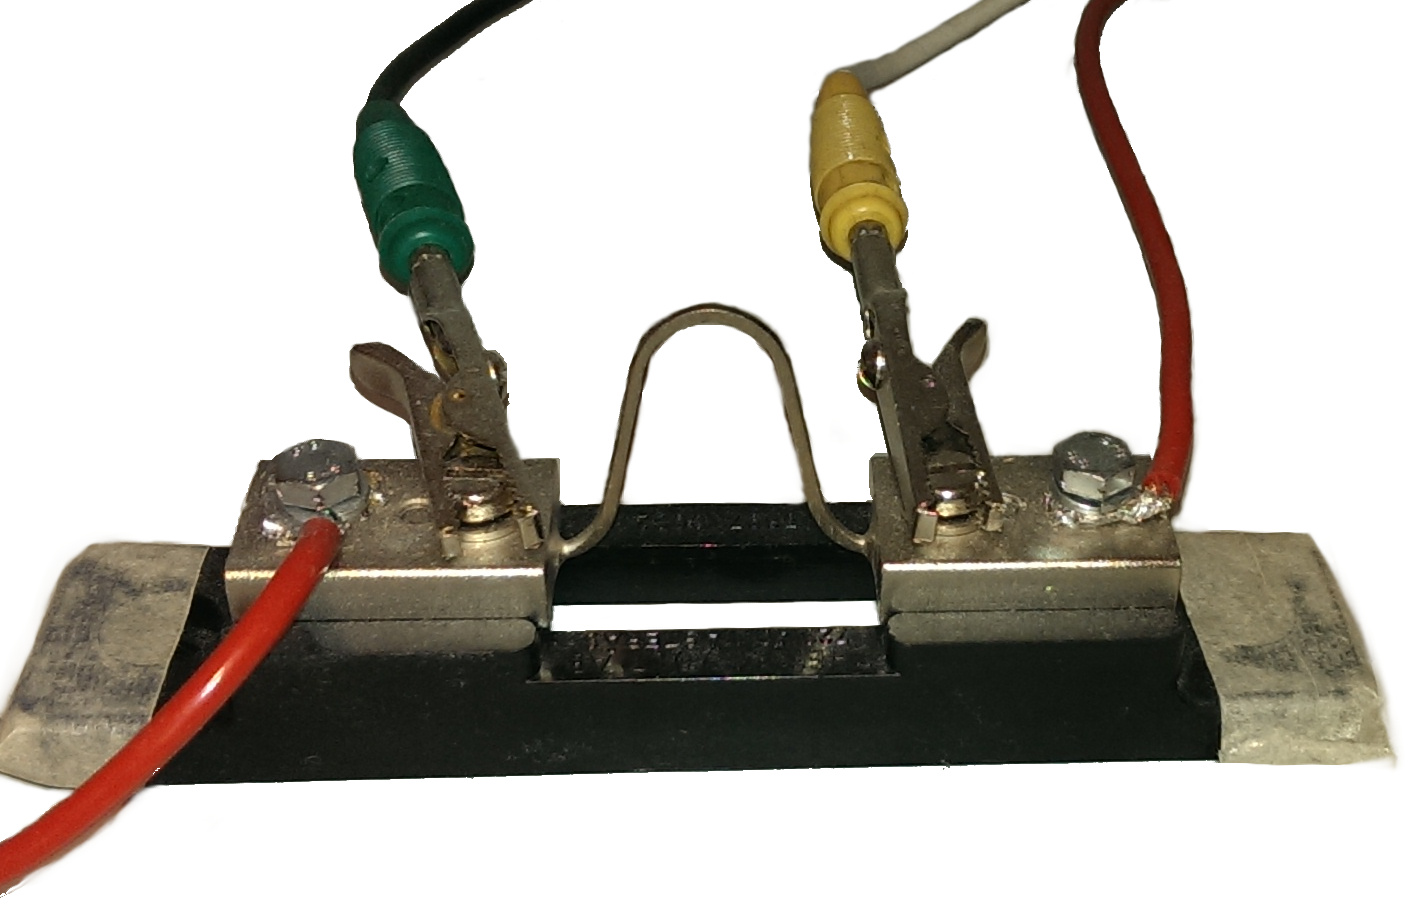
\includegraphics[width=0.8\textwidth]{figs/shunt.jpg}
    \caption{An example shunt resistor}
    \label{fig:shunt}
\end{figure}

% TODO: Where does this fit?
% The ultimate goal in this context is to estimate power consumption and energy
% efficiency of new hardware, the first step is to measure different more or less
% power consuming events on real hardware that is similar to the one simulated.

